
\section{现有智能体推理系统面临的挑战}
\label{sec:motivation}
\begin{figure*}[t!]  % 使用 figure* 让图片跨越两栏
    \centering
    \begin{subfigure}{0.32\textwidth}
        \centering
        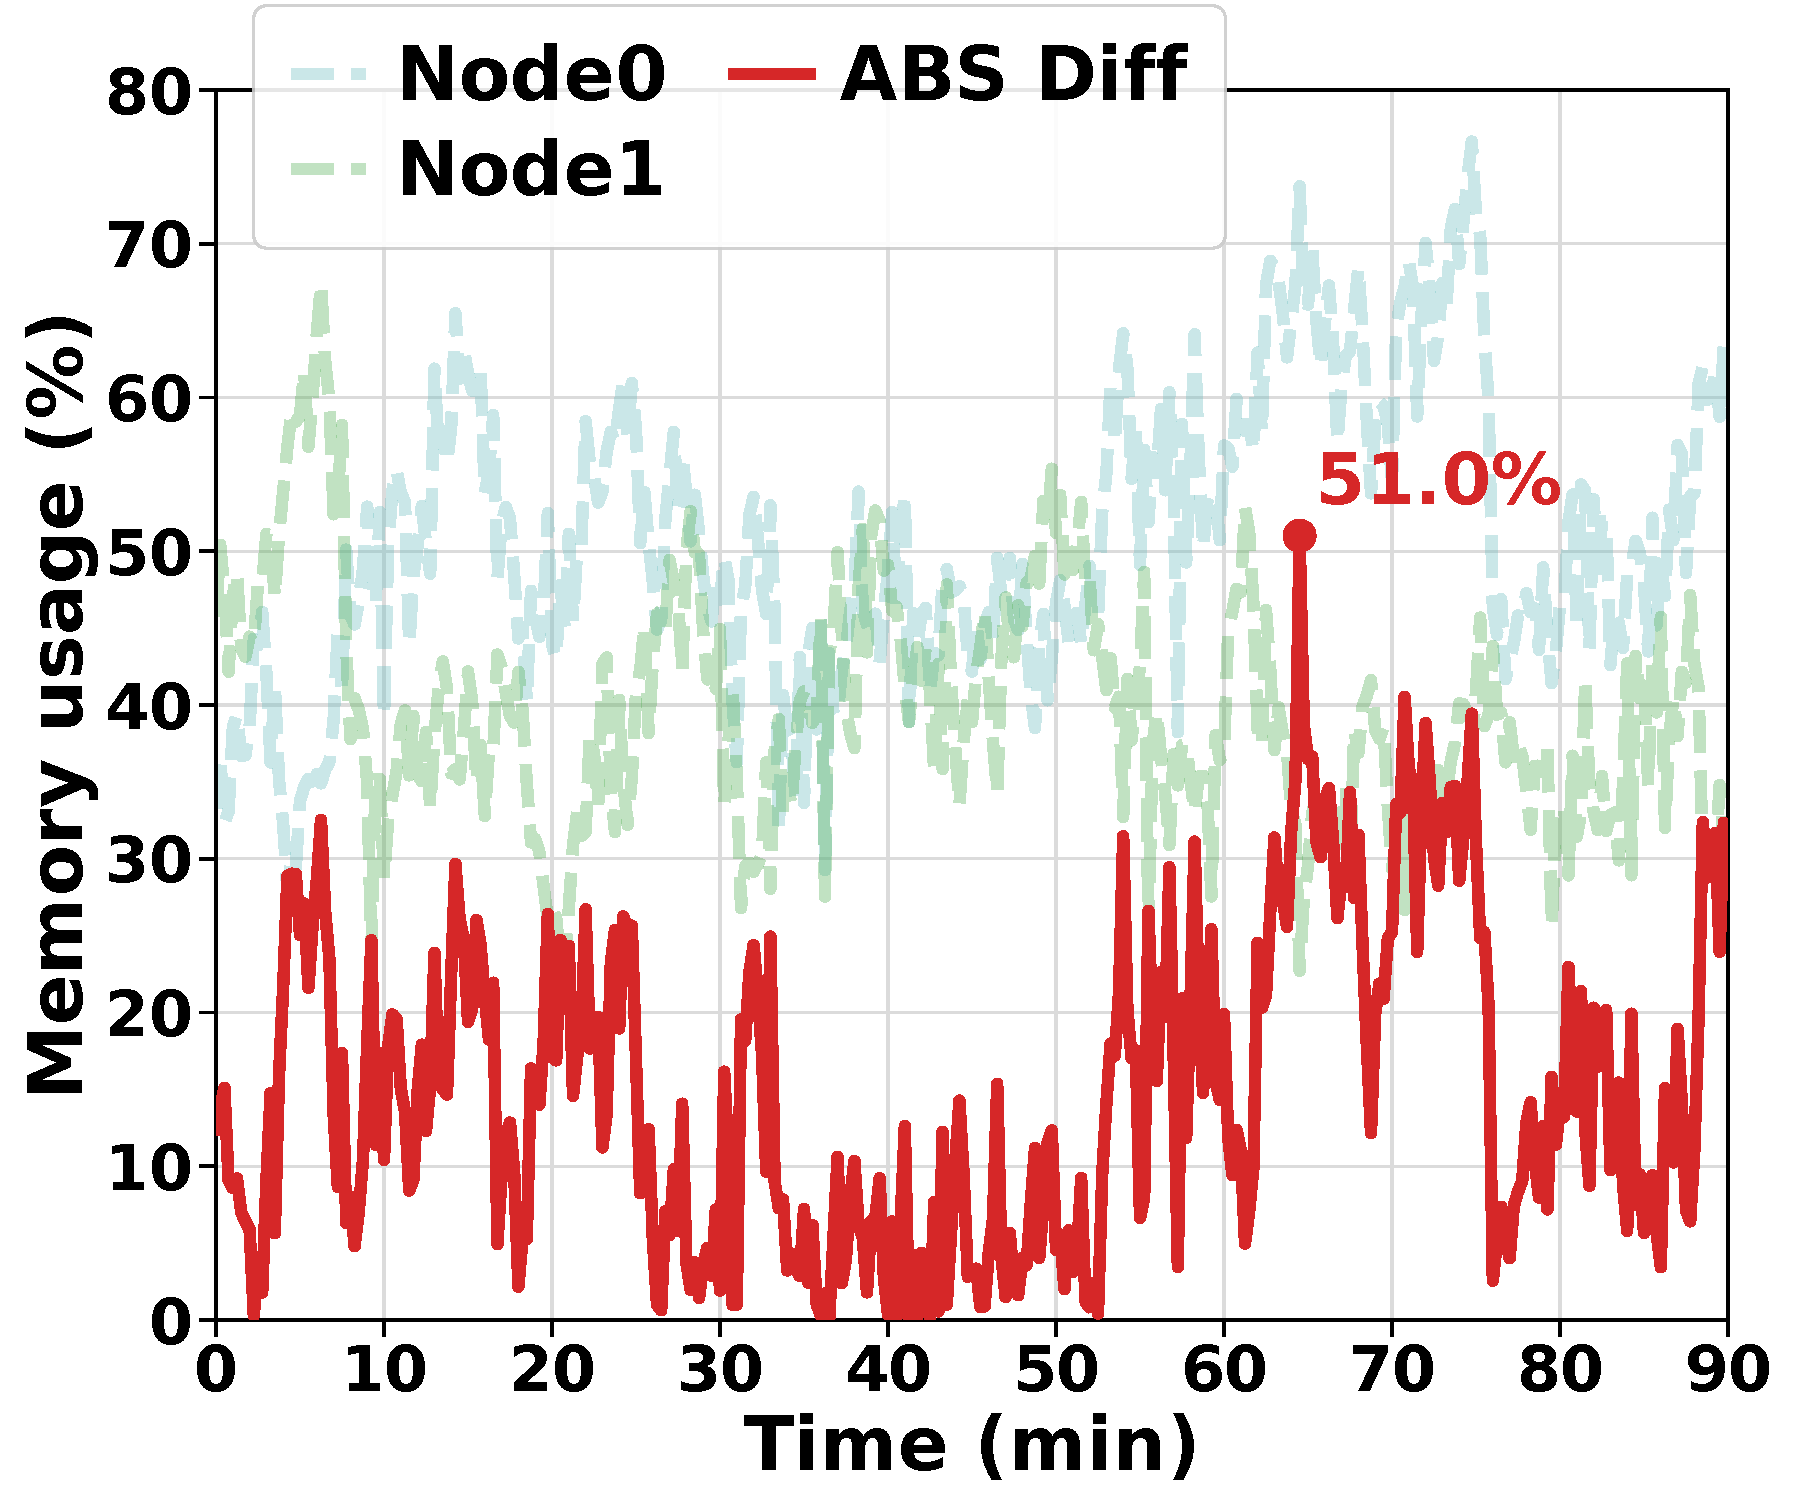
\includegraphics[width=\textwidth]{Figures/unbalance_memory_vs_time.pdf}  % 替换为你的图片路径
        \caption{部署时显存不均衡}
        \label{fig:dp unbalance}
    \end{subfigure}
    \begin{subfigure}{0.32\textwidth}
        \centering
        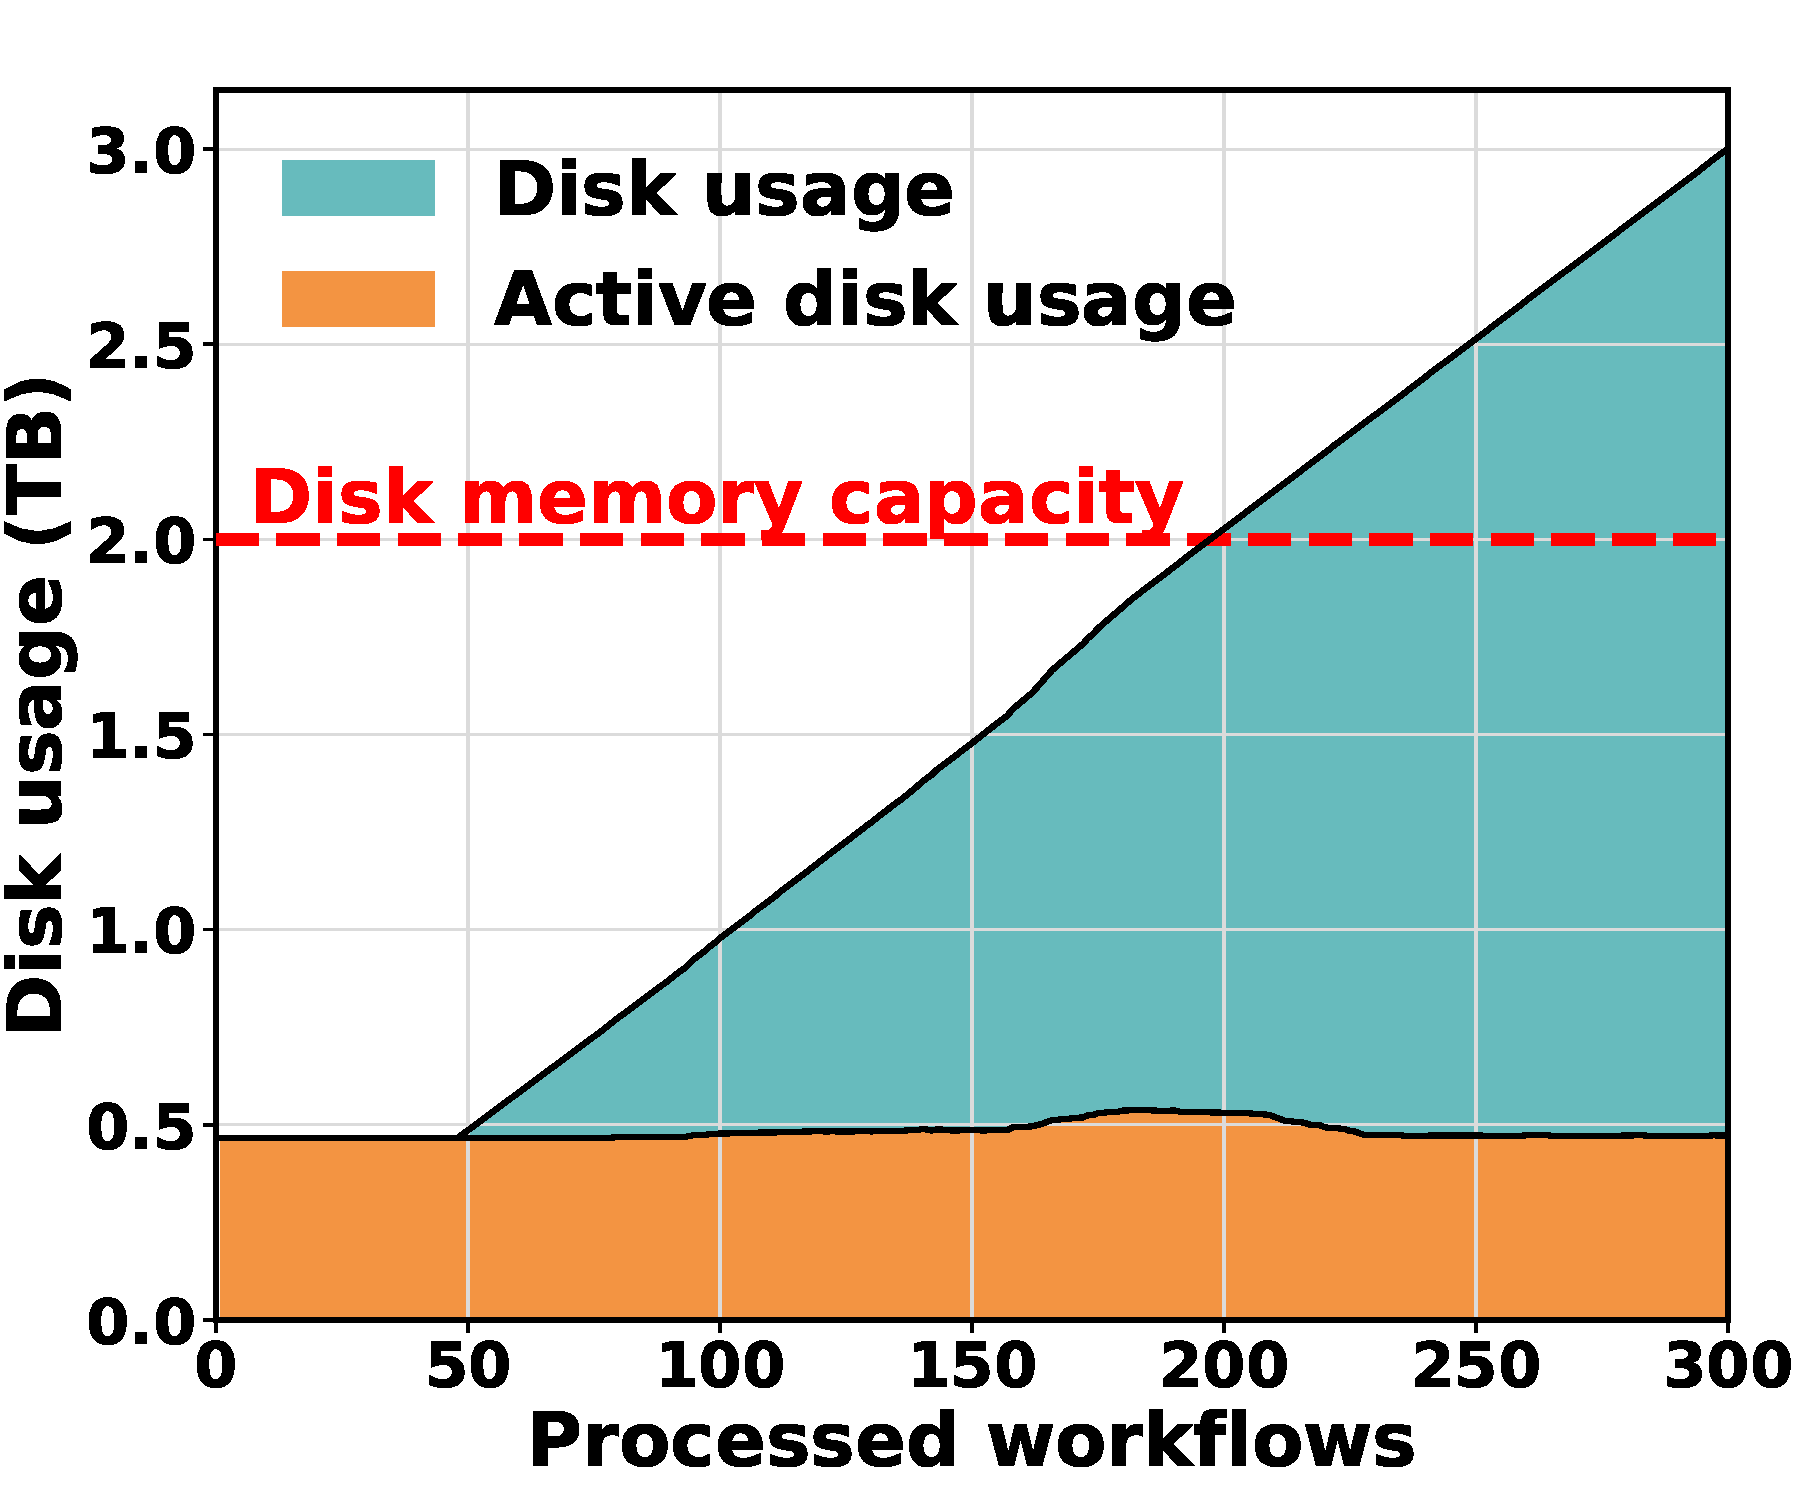
\includegraphics[width=\textwidth]{Figures/disk_usage_vs_instance_number.pdf}  % 替换为你的图片路径
        \caption{工具环境的运行时磁盘使用情况。}
        \label{fig:disk mem}
    \end{subfigure}
    \begin{subfigure}{0.32\textwidth}
        \centering
        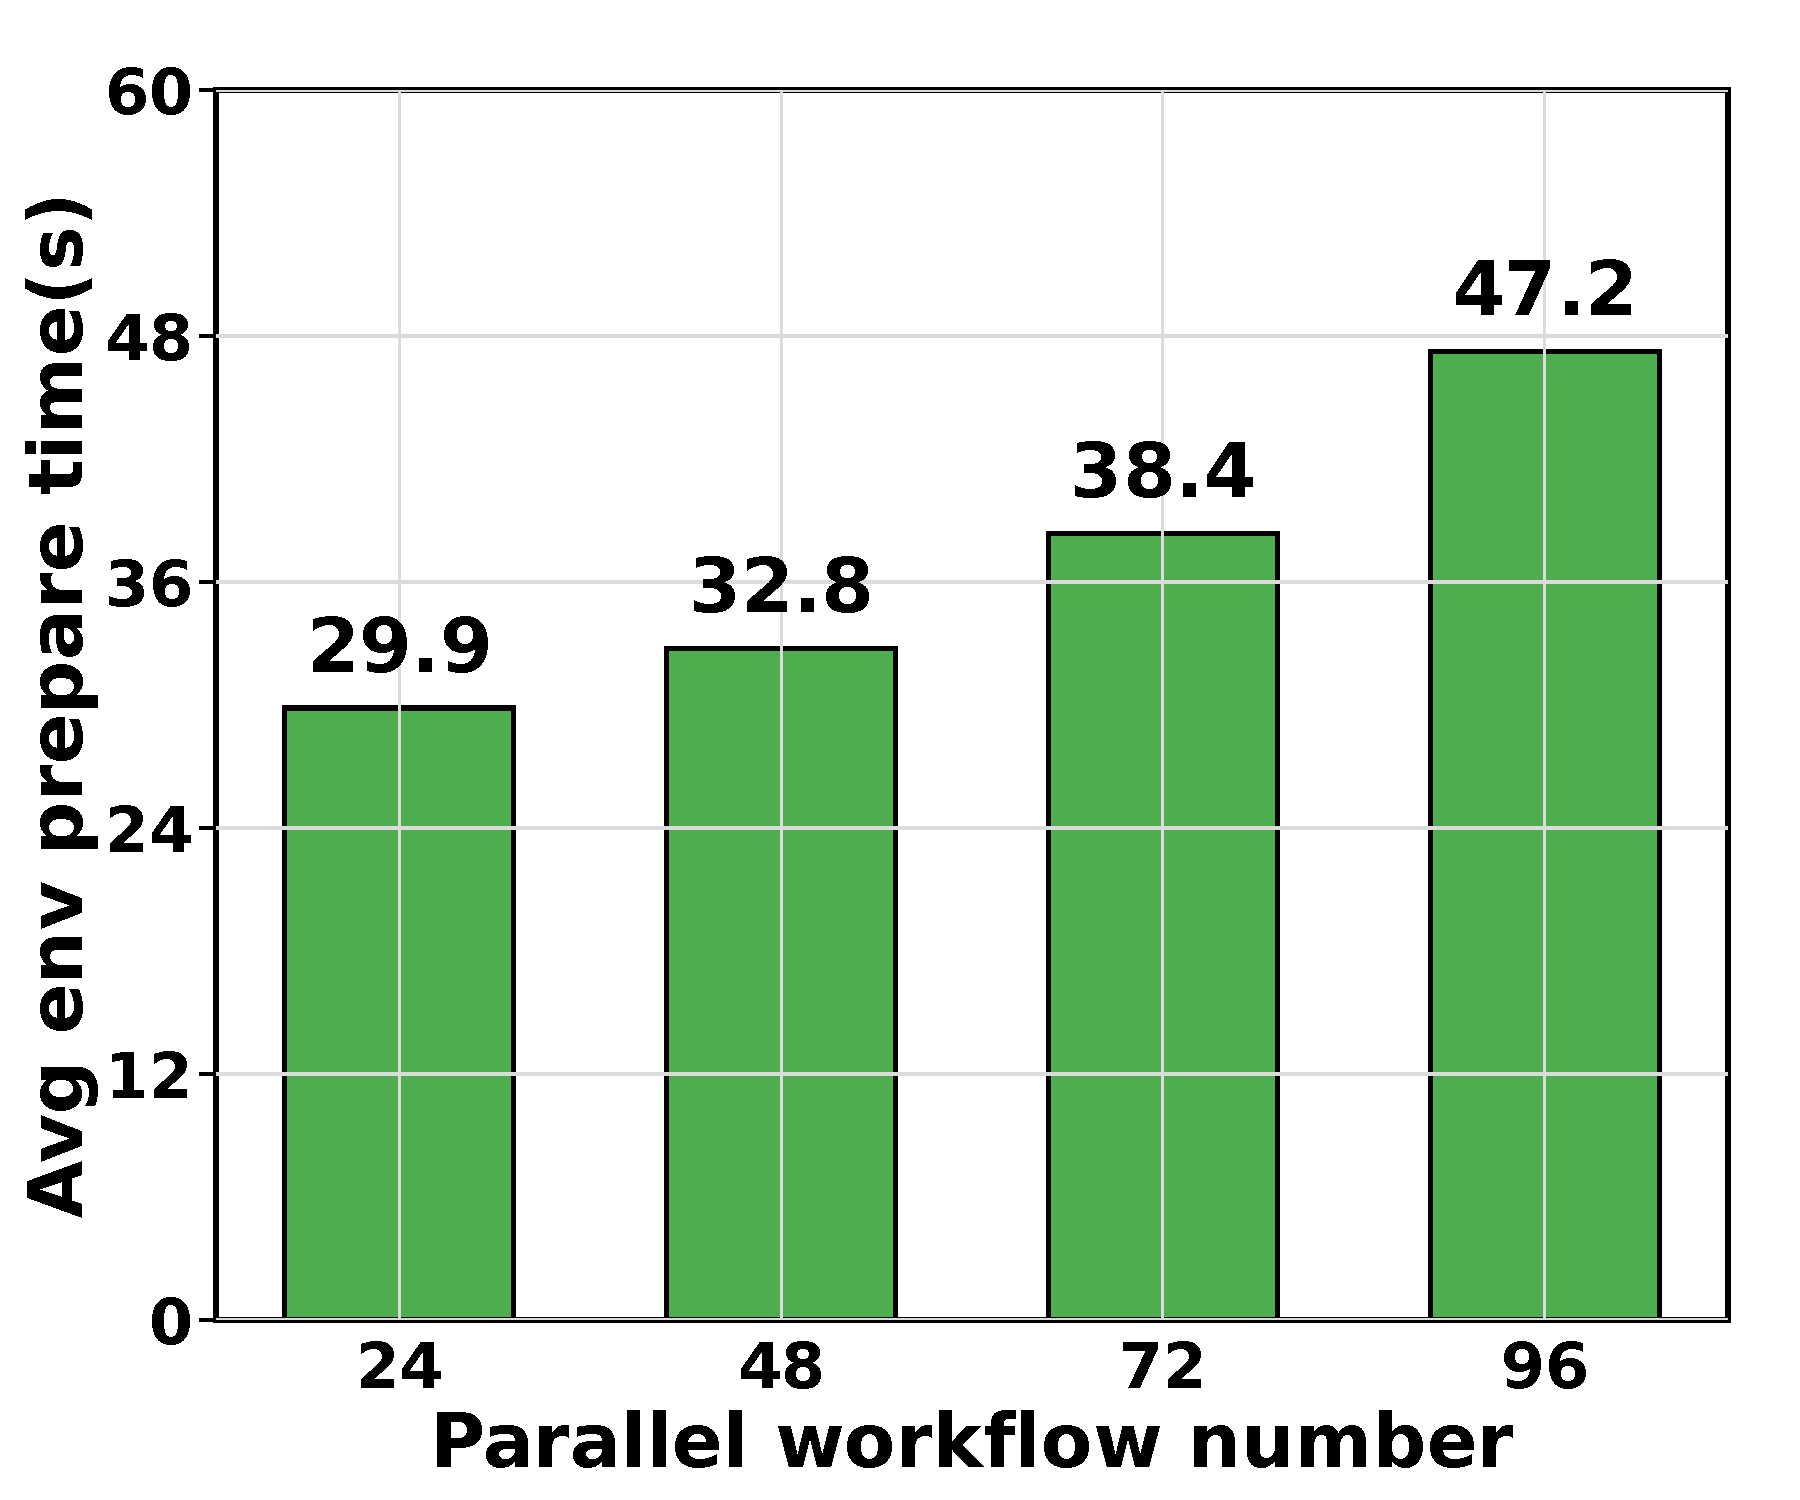
\includegraphics[width=\textwidth]{Figures/env_prepare_vs_bs.pdf}  % 替换为你的图片路径
        \caption{工具环境准备时间}
        \label{fig:env prepare}

    \end{subfigure}
    \caption{\textbf{当前智能体推理系统中的显存不均衡和工具资源管理问题。} 我们在 OpenHands RL rollout 上评估 vLLM + Kubernetes，使用 SWE-Bench-Lite 上的 GLM-4.6 模型和两个 8$\times$H100 GPU 节点。观察结果表明：(a) 应用 vLLM KV 感知路由器时，在 90 分钟 rollout 测试中最大显存不均衡可达到 51\%；(b) 工具执行环境垃圾回收失败会逐渐导致资源使用超过系统容量；(c) \mbox{随着并行工作流数量增加，平均工具执行环境准备时间快速增长。}}
    \label{fig:3}
    \vspace{-2mm}
\end{figure*}



本节以 vLLM 与 Kubernetes 的组合作为多轮智能体推理的代表性基线，并总结其中的关键低效问题。值得注意的是，这些限制并不能仅通过替换推理引擎（例如 TensorRT 或 SGLang）或工具编排器解决，而是需要新的程序感知抽象。默认设置下，我们使用 GLM-4.6 模型，在两个 8$\times$H100 GPU 节点上运行 OpenHands RL rollout。
% We use vLLM with Kubernetes as our request-aware agentic inference baseline.
\vspace{-2mm}
\subsection{KV 缓存抖动}
\label{sec:kv cache management}
% \textbf{KV-cache thrashing.} As discussed in \Cref{sec::react agent system}, current agents exhibit a high theoretical KV-cache reuse ratio throughout their execution. However, in high-concurrency scenarios, typical of large-batch serving and RL rollouts, the GPU memory allocated to a workload's state is frequently preempted during its tool-acting phase. Because standard serving engines treat the acting interval as an idle period, the associated KV cache is often evicted to accommodate other active requests.

% As discussed in~\Cref{sec::react agent system}, a
智能体工作流在执行期间具有较高的理论 KV 缓存重用率。然而，在现有 LLM 服务系统中，每一步都作为独立且无状态的请求处理。在高并发下，这种请求级调度会导致 KV 缓存在工具执行期间频繁被驱逐，以容纳新到达的请求；随之而来的重复驱逐和重新预填充就是 KV 缓存抖动。

%However, under high concurrency, inference systems suffer frequent evictions, a phenomenon we refer to as KV cache thrashing.
% of agentic workflows is often evicted to accommodate other workflows' active requests.

如图所示 \Cref{fig:workload_profile}，随着并行工作流数量增加，这种抖动会加剧。由此导致的缓存命中率下降会触发频繁且成本高昂的重新预填充，系统必须在工具完成后重新计算整个历史记录。与非抖动设置相比，这种冗余会使每个请求的端到端延迟最高增加 \textbf{7.14$\times$}，并导致吞吐量严重下降。

% Because request-centric engines lack visibility into the agent's execution phase, they treat these tool-execution intervals as idle periods, allowing other programs to evict existing context under memory pressure. This leads to severe GPU memory thrashing, where programs are forced to continuously re-prefill their history once tool execution concludes. As illustrated in \autoref{fig:kv thrashing}, an increase in parallel programs correlates with a sharp decline in the average KV-cache hit rate and a significant escalation in per-request prefill latency.
\vspace{-2mm}
\subsection{跨节点显存不均衡}
\label{sec:cross node imbalance}
当前跨数据并行（DP）节点路由请求的策略也并非最优。现有多轮调度器~\citep{zheng2024sglangefficientexecutionstructured, vllm_kvaware_routing} 会贪婪地把请求分配给 KV 缓存局部性最高的目标 DP 节点，以最大化缓存重用。然而，该策略忽略了节点之间显存负载可能变得不均衡这一事实。例如，vLLM 中的 KV 感知路由器~\citep{vllm_kvaware_routing} 会将来自同一智能体工作流的所有请求发送到同一节点。由于不同工作流可能具有高度异构的 KV 占用和执行生命周期，这种策略常常导致节点之间严重显存不均衡：一些节点过载，而其他节点利用率较低。类似地，SGLang 中的前缀感知路由器会贪婪地把工作负载路由到具有匹配前缀的节点，以最大化缓存命中率。由于智能体系统提示在工作流中相同，该策略会把几乎所有请求发送到同一节点，同时让其他节点空闲。


如图所示 \Cref{fig:dp unbalance}，在智能体 RL rollout 的 90 分钟快照中，两个 DP 节点之间的显存使用差距有超过 37 分钟 \textbf{大于 20\%}，峰值不均衡达到 51\%。
% because workloads can not transfer between nodes.
 % \textbf{ Distributed agentic scheduler should dynamically balance KV-cache locality and memory balancing across nodes.}

\subsection{工具生命周期的遗忘}
\label{sec:Tool mismanagement}
当前的智能体推理系统不将外部工具编排器的生命周期与 LLM推理引擎同步，从而导致工具编排器端的无声资源浪费和延迟开销。

\paragraph{资源泄漏和未使用的沙箱。}
% Most tool resources are shared across requests within a workflow.
% , and their lifecycles are identical to the workflow as well.
% However, modern inference systems lack native mechanisms to synchronize these lifecycles.
\vspace{-2mm}
\Cref{fig:disk mem} 展示了总磁盘空间占用随着处理的工作流数量线性增加，最终超过系统容量。这是因为工作流完成时未回收未使用的资源（例如已完成工作负载的 Docker 映像）。这种低效的垃圾收集会导致长期智能体推理的致命系统不稳定。

\paragraph{昂贵的环境准备。}
我们观察到，大多数智能体工作负载需要在启动多轮轨迹之前准备环境。例如，编码智能体需要拉取docker、安装相关包并构建存储库。此外，这种准备时间成本高昂，并且随着并行工作负载数量（即批量大小）的增加而增加，如图所示 \Cref{fig:env prepare}。如果 LLM推理引擎需要等到环境完全准备好，这种开销将延长推理系统的端到端延迟。

% These inefficiencies highlight the necessity of a \textbf{unified system abstraction} that captures all heterogeneous resources.

% Most of the tools currently used by agents are either shared by request in the same workload. For those tool resources, the lifecycle is the same as the workload. For example, sandboxes or ip address connected to the database or retriever should be collected and deleted or released after the workload is terminated. However, current inference systems are not natively embedded with such mechanisms. Shown in \autoref{fig:disk mem}, the total disk memory continue to increases with the processed program and exceeded the disk memory capacity of the system. However, disk memory used by processing program is only part of the total occupied memory. Unefficient garbage collection is extremely harmful to long time serving and will triggers Out-of-Memory (OOM) errors and system instability.


% \begin{figure}[t!]  % 使用 figure* 让图片跨越两栏
%     \centering

%         \centering
%         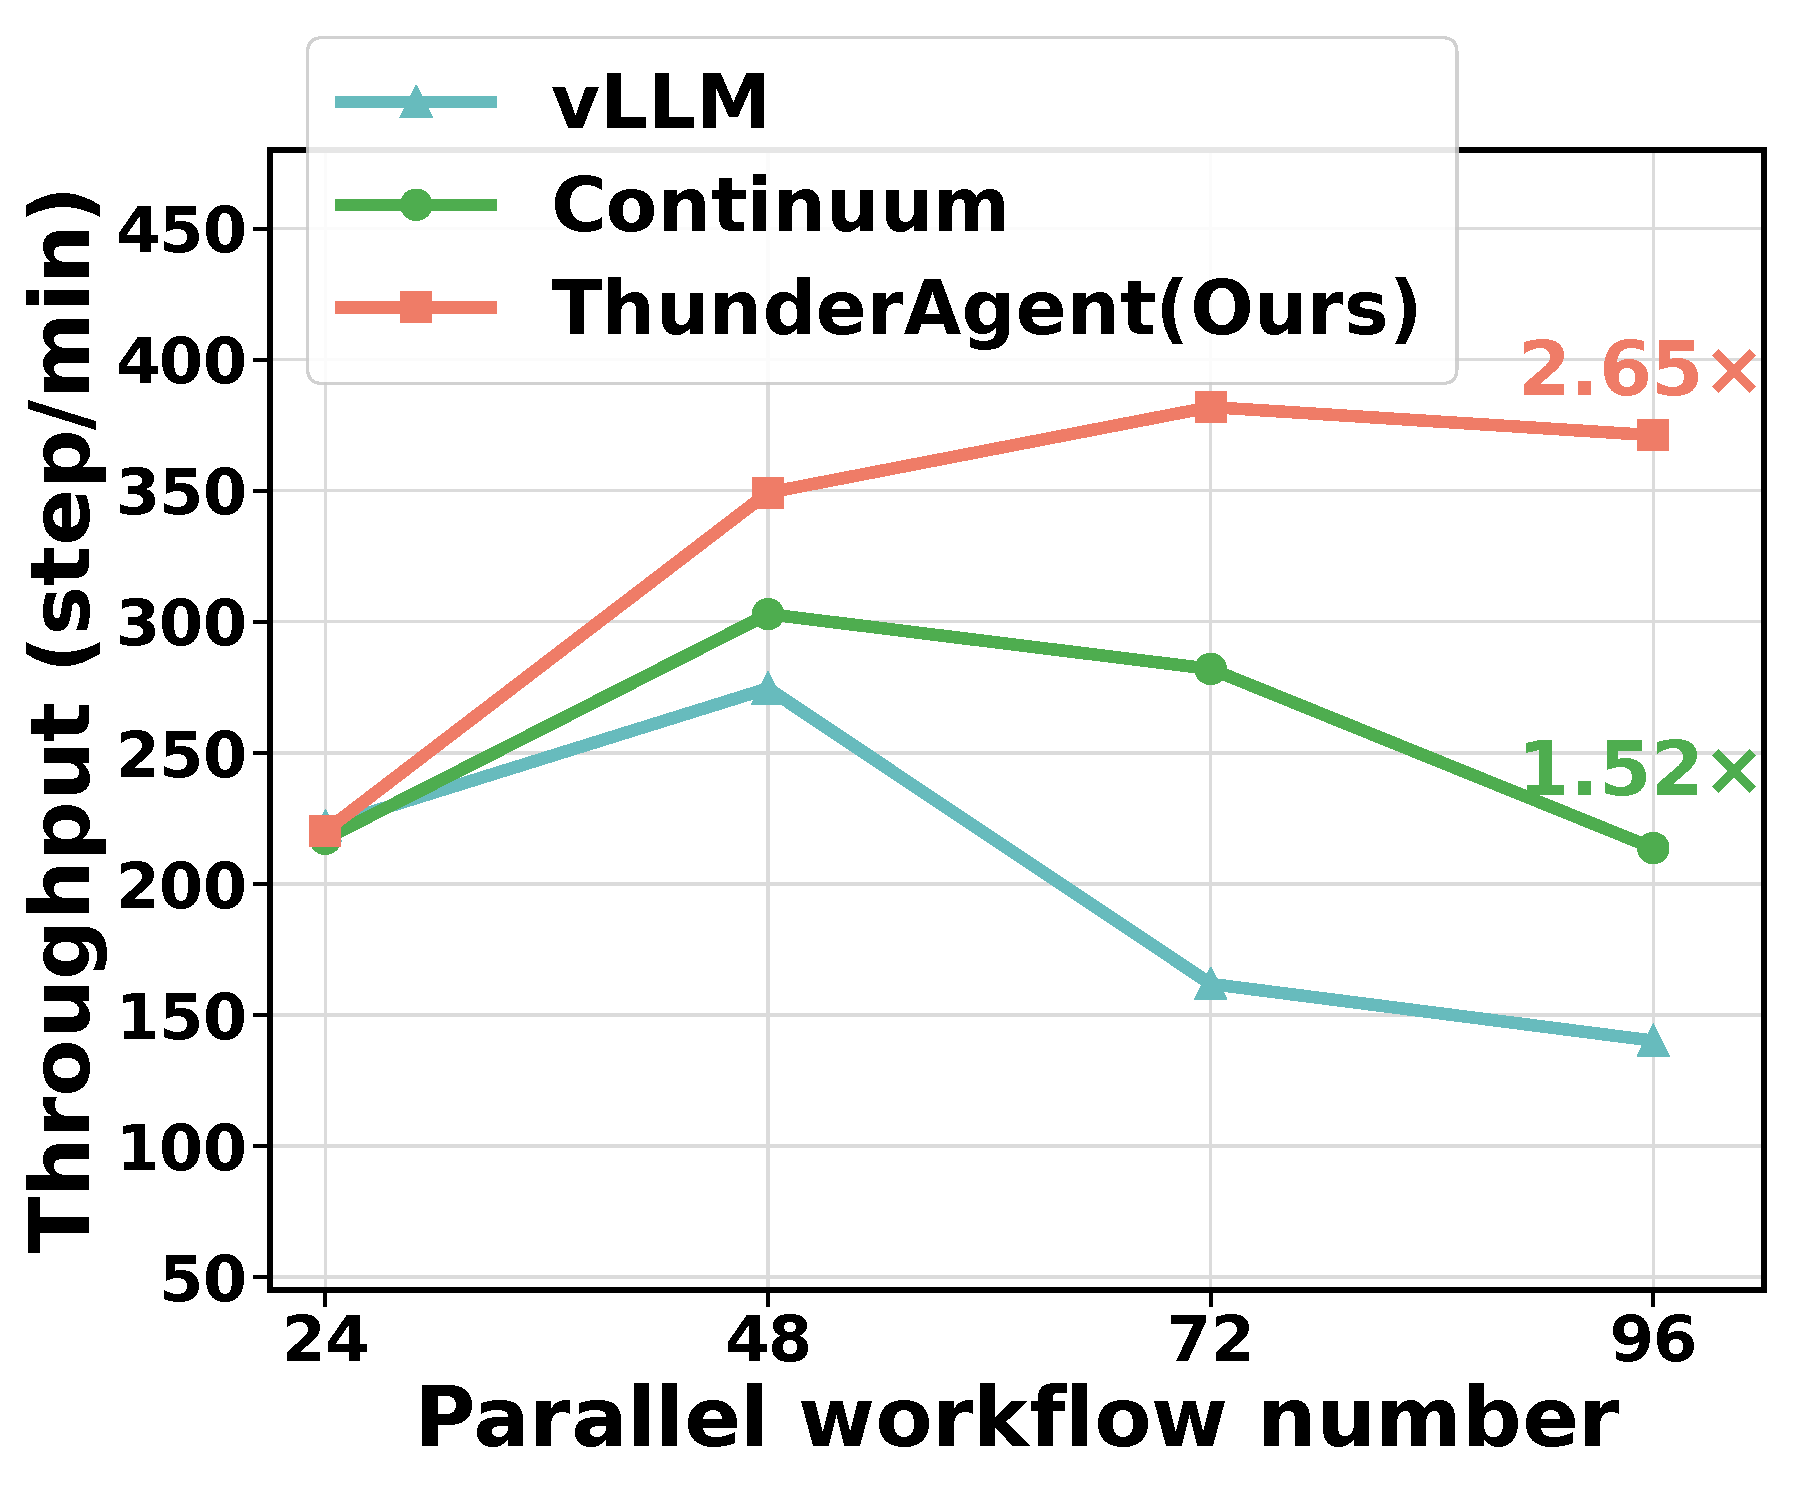
\includegraphics[width=0.32\textwidth]{Figures/throughputs_vs_bs.pdf}  % 替换为你的图片路径
%         \caption{TBD}


%     \label{fig:kv thrashing}
% \end{figure}

% \begin{figure}[t!]  % 使用 figure* 让图片跨越两栏
%     \centering

%         \centering
%         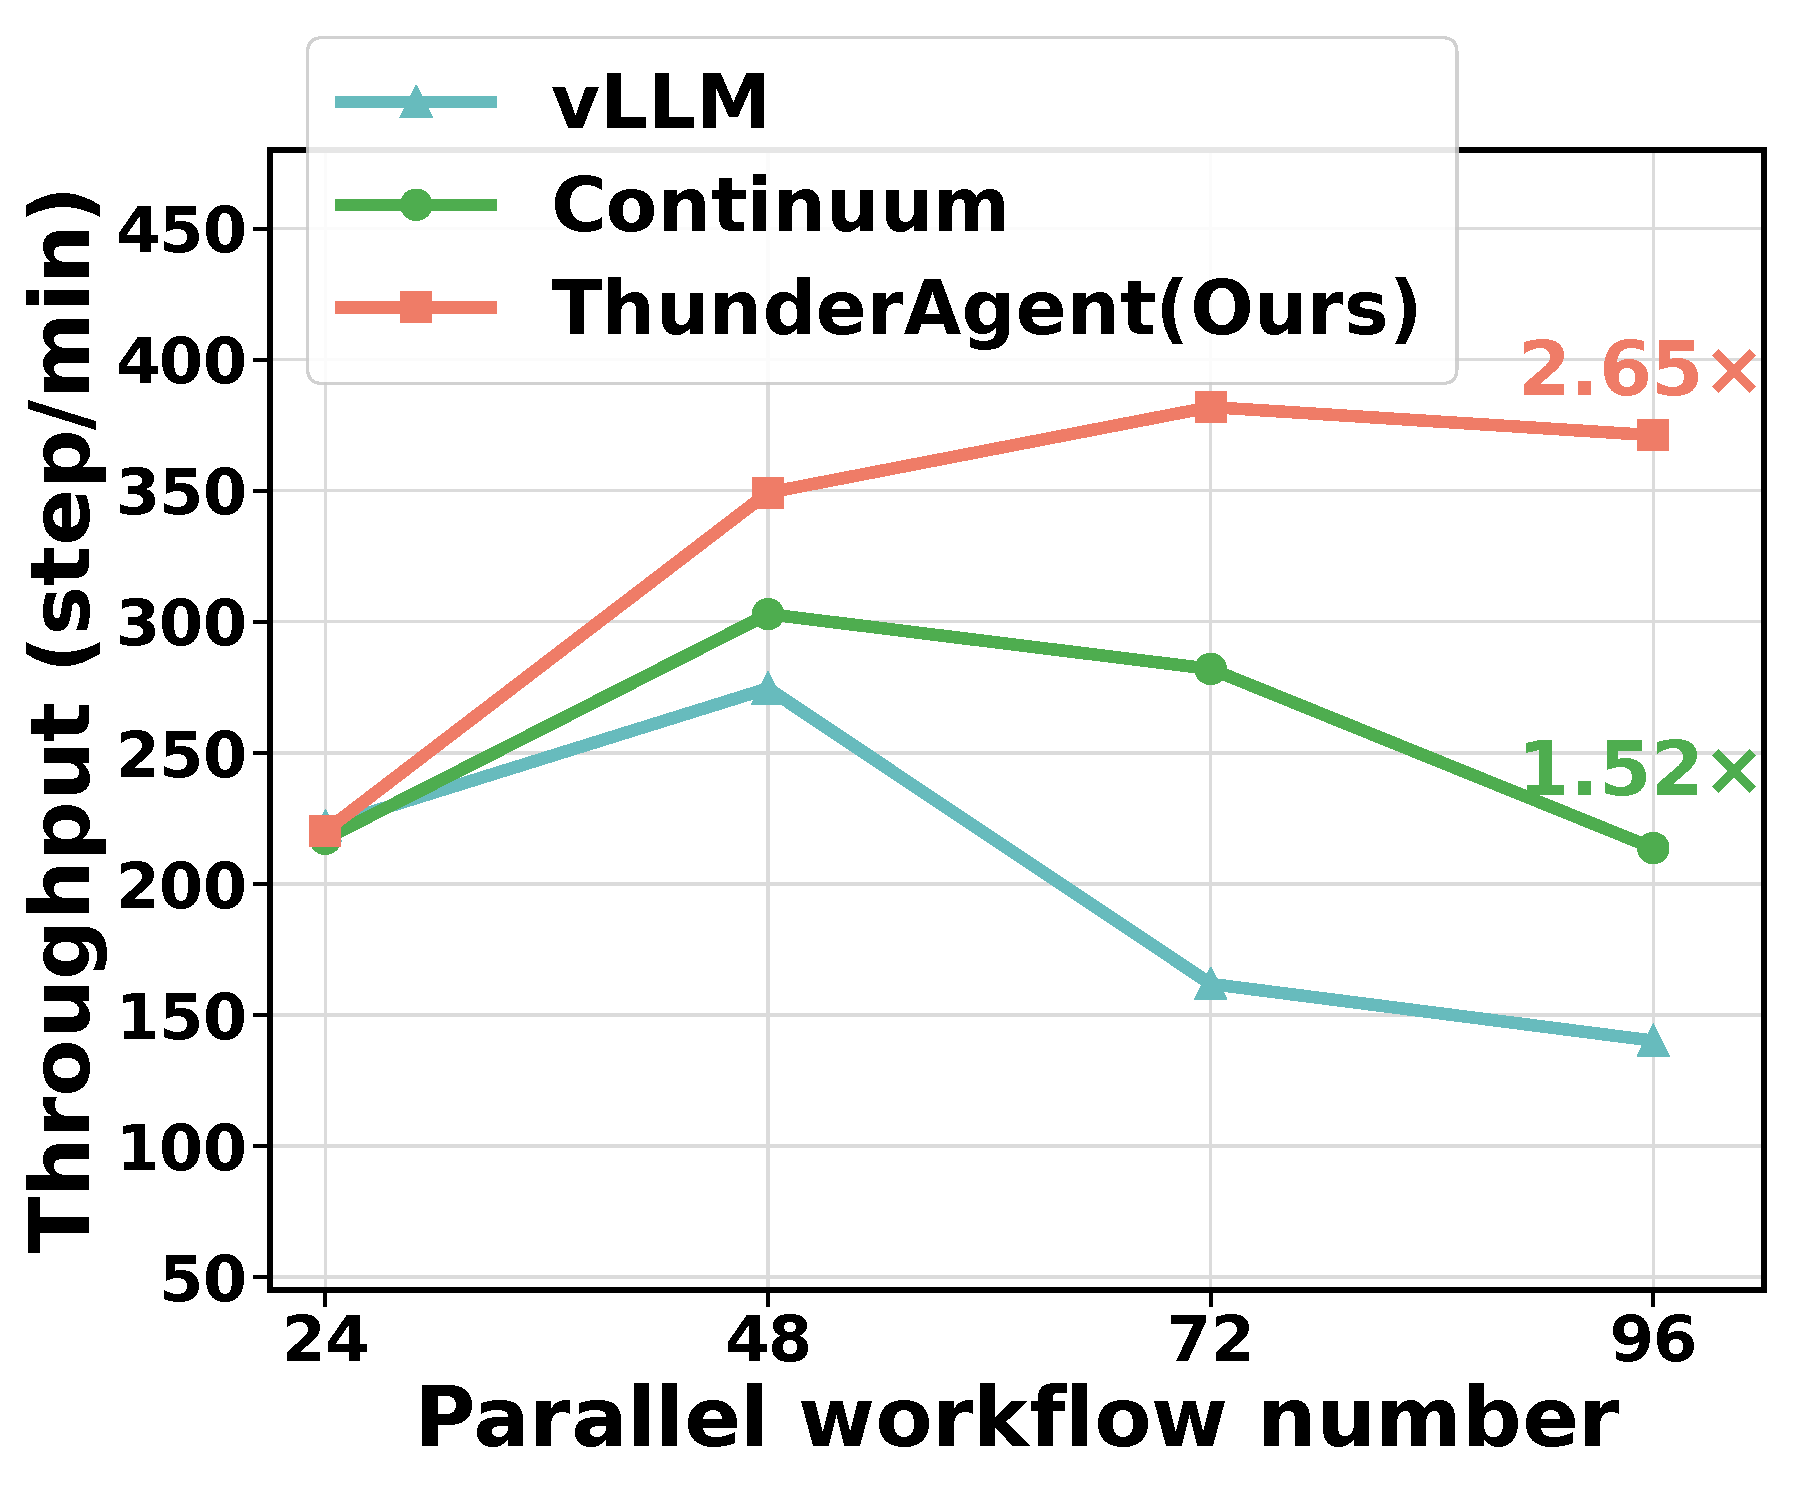
\includegraphics[width=0.32\textwidth]{Figures/throughputs_vs_bs.pdf}  % 替换为你的图片路径
%         \caption{TBD}


%     \label{fig:DP unbalance}
% \end{figure}

% \subsection{Incomplete Mismanagement for Tool Lifecycle}
